\documentclass{beamer}
%\usetheme{Warsaw}
%\beamersetaveragebackground{brown!25}
\usetheme{Warsaw}
\usecolortheme[rgb={0.6,0.18,0.11}]{structure}

\newtheorem{tw}{Twierdzenie}


\usepackage[font=scriptsize, labelfont=bf]{caption}
\usepackage{latexsym,amsmath}
\usepackage{graphicx}
\usepackage[T1]{fontenc}
\usepackage[cp1250]{inputenc}
%\usepackage[MeX]{polski}
%\usepackage[utf8]{inputenc}
\setbeamertemplate{navigation symbols}{}
%\usepackage{beamerthemesplit}
\title[Korygowanie harmonogram�w z uwzgl�dnieniem awarii ...]{Korygowanie harmonogram�w\\ z uwzgl�dnieniem awarii maszyn}
\author{Kamil Niemczyk}
\institute{Politechnika Wroc�awska\\ Automatyka i Robotyka, Wydzia� Elektroniki\\ Technologie informacyjne w systemach
automatyki}


\date{
\includegraphics[width=18mm]{pwr.jpg}}

\newcommand{\tab}{\hspace*{1cm}}
\newcommand{\ta}{\hspace*{5mm}}
\newcommand{\tas}{\hspace*{8mm}}
\newcommand{\tat}{\hspace*{4mm}}

\newcommand*\oldmacro{}
\let\oldmacro\insertshortauthor% save previous definition
\renewcommand*\insertshortauthor{%
  \leftskip=.3cm% before the author could be a plus1fill ...
  \insertframenumber\,/\,\inserttotalframenumber\hfill\oldmacro}

\begin{document}
\setbeamercovered{transparent=15}
%\setbeamertemplate{footline}[frame number]
\begin{frame}
\maketitle
\end{frame}

\begin{frame}
\frametitle{Plan prezentacji} \tableofcontents

Zaproponowano algorytm Tabu Search z nawrotami, kt�ry przystosowano do rozwi\k{a}zywania elastycznych problem�w gniazdowych.
\end{frame}




\section{Korygowanie harmonogram�w z uwzgl�dnieniem zak��ce�}

\begin{frame}
\frametitle{Elastyczny problem gniazdowy}

Let us consider
\begin{itemize}
\item ${J} = {\{}1, 2, \ldots, n${\}} -- a set of jobs, \item $M =
{\{}1, 2, \ldots, m${\}} -- a set of machines, \item ${O} = {\{}1,
2, \ldots, o${\}} -- a set of operations.
\end{itemize}

A job $j$ consists of the sequence of $o_{j}$ operations. An
operation $i$ has to be executed on the dedicated machine without
interruptions in time $p_{i}
> 0$, $i \in {O}$. The solution is a vector of times $S $= ($S_{1}$, $S_{2}$, \ldots, $S_{o})$ of operations beginning such, that:
\begin{itemize}
\item a job begins its execution on the next machine if it is
finished on the previous one,

\item a job begins on the machine if the previous job executed on
this machine is finished,

\item beginning times are not negative.
\end{itemize}

\end{frame}


\subsection{Mathematical model}

\begin{frame}
\frametitle{The job shop problem}


A feasible solution: a vector $S $= ($S_{1}$, $S_{2}$, \ldots, $S_{o})$ such, that: 
$$
S_{l_{j - 1} + 1} \ge 0,\quad j = 1, 2, \ldots, n,
$$
$$
S_{i} + p_{i} \le S_{i + 1}, \;\; i = l_{j - 1} + 1,\;\; l_{j - 1}
+ 2, \ldots, l_{j} - 1, \;\; j = 1, 2, \ldots, n,
$$
$$S_{i} + p_{i} \le  S_{j} \quad\textnormal{or}\quad S_{j} + p_{j}
\le S_{i}, \quad i,j  \in  O, \quad v_{i} = v_{j}, \quad i \ne j.
$$
where $C_j = S_j + p_j$, a machine number $v_i$ of a job $i$. 
 
\begin{center}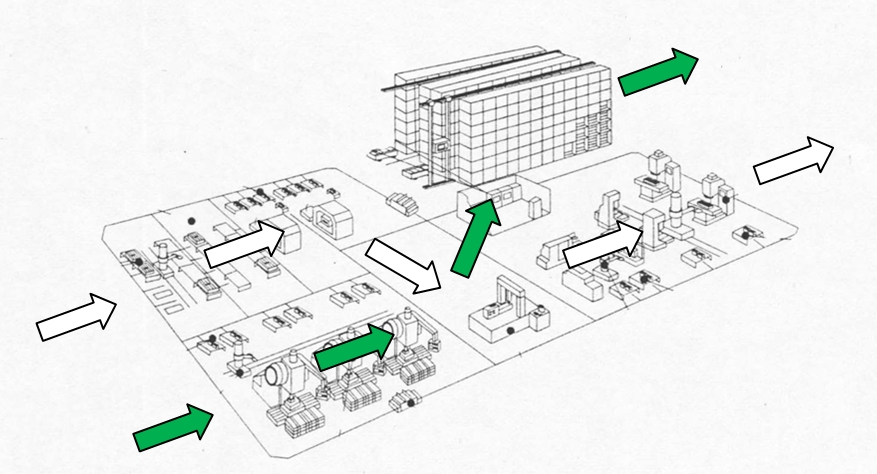
\includegraphics[width=6cm]{Fabryka_Strzalki.jpg}\end{center}

\end{frame}


\subsection{Cost function}

\begin{frame}
\frametitle{The job shop problem}

An appropriate criterion function
has to be added to the problem constraints: 
\begin{itemize}
\item minimization of the time of finishing
all the jobs
$$
C_{\max } (S) = \mathop {\max }\limits_{1 \le j \le n} C_{l_j},
$$
\item minimization of the sum of job
finishing times
%
$$
C(S) = \sum\limits_{j = 1}^n C_{l_j }.
$$
\end{itemize}
Both problems described are strongly NP-hard\index{NP-hard
problem} and although they are similarly modelled, the second one
is found to be harder because of the lack of some specific
properties (so-called block properties).

\end{frame}

\section{Tabu search with neural network}

\subsection{Neighborhood}

\begin{frame}
\frametitle{Neighborhood}

In the considered neuro-tabu search algorithm $NTS$ each move is represented
by its neuron. For the adjacent swap neighborhood a
network of neurons formed of $o-1$ neurons. Let $i$-th neuron
represents a move consisting in swap of two adjacent elements on
the positions $i$ and $i+1$ in a solution~$\pi$.

\begin{figure}[!h]
    \centering
    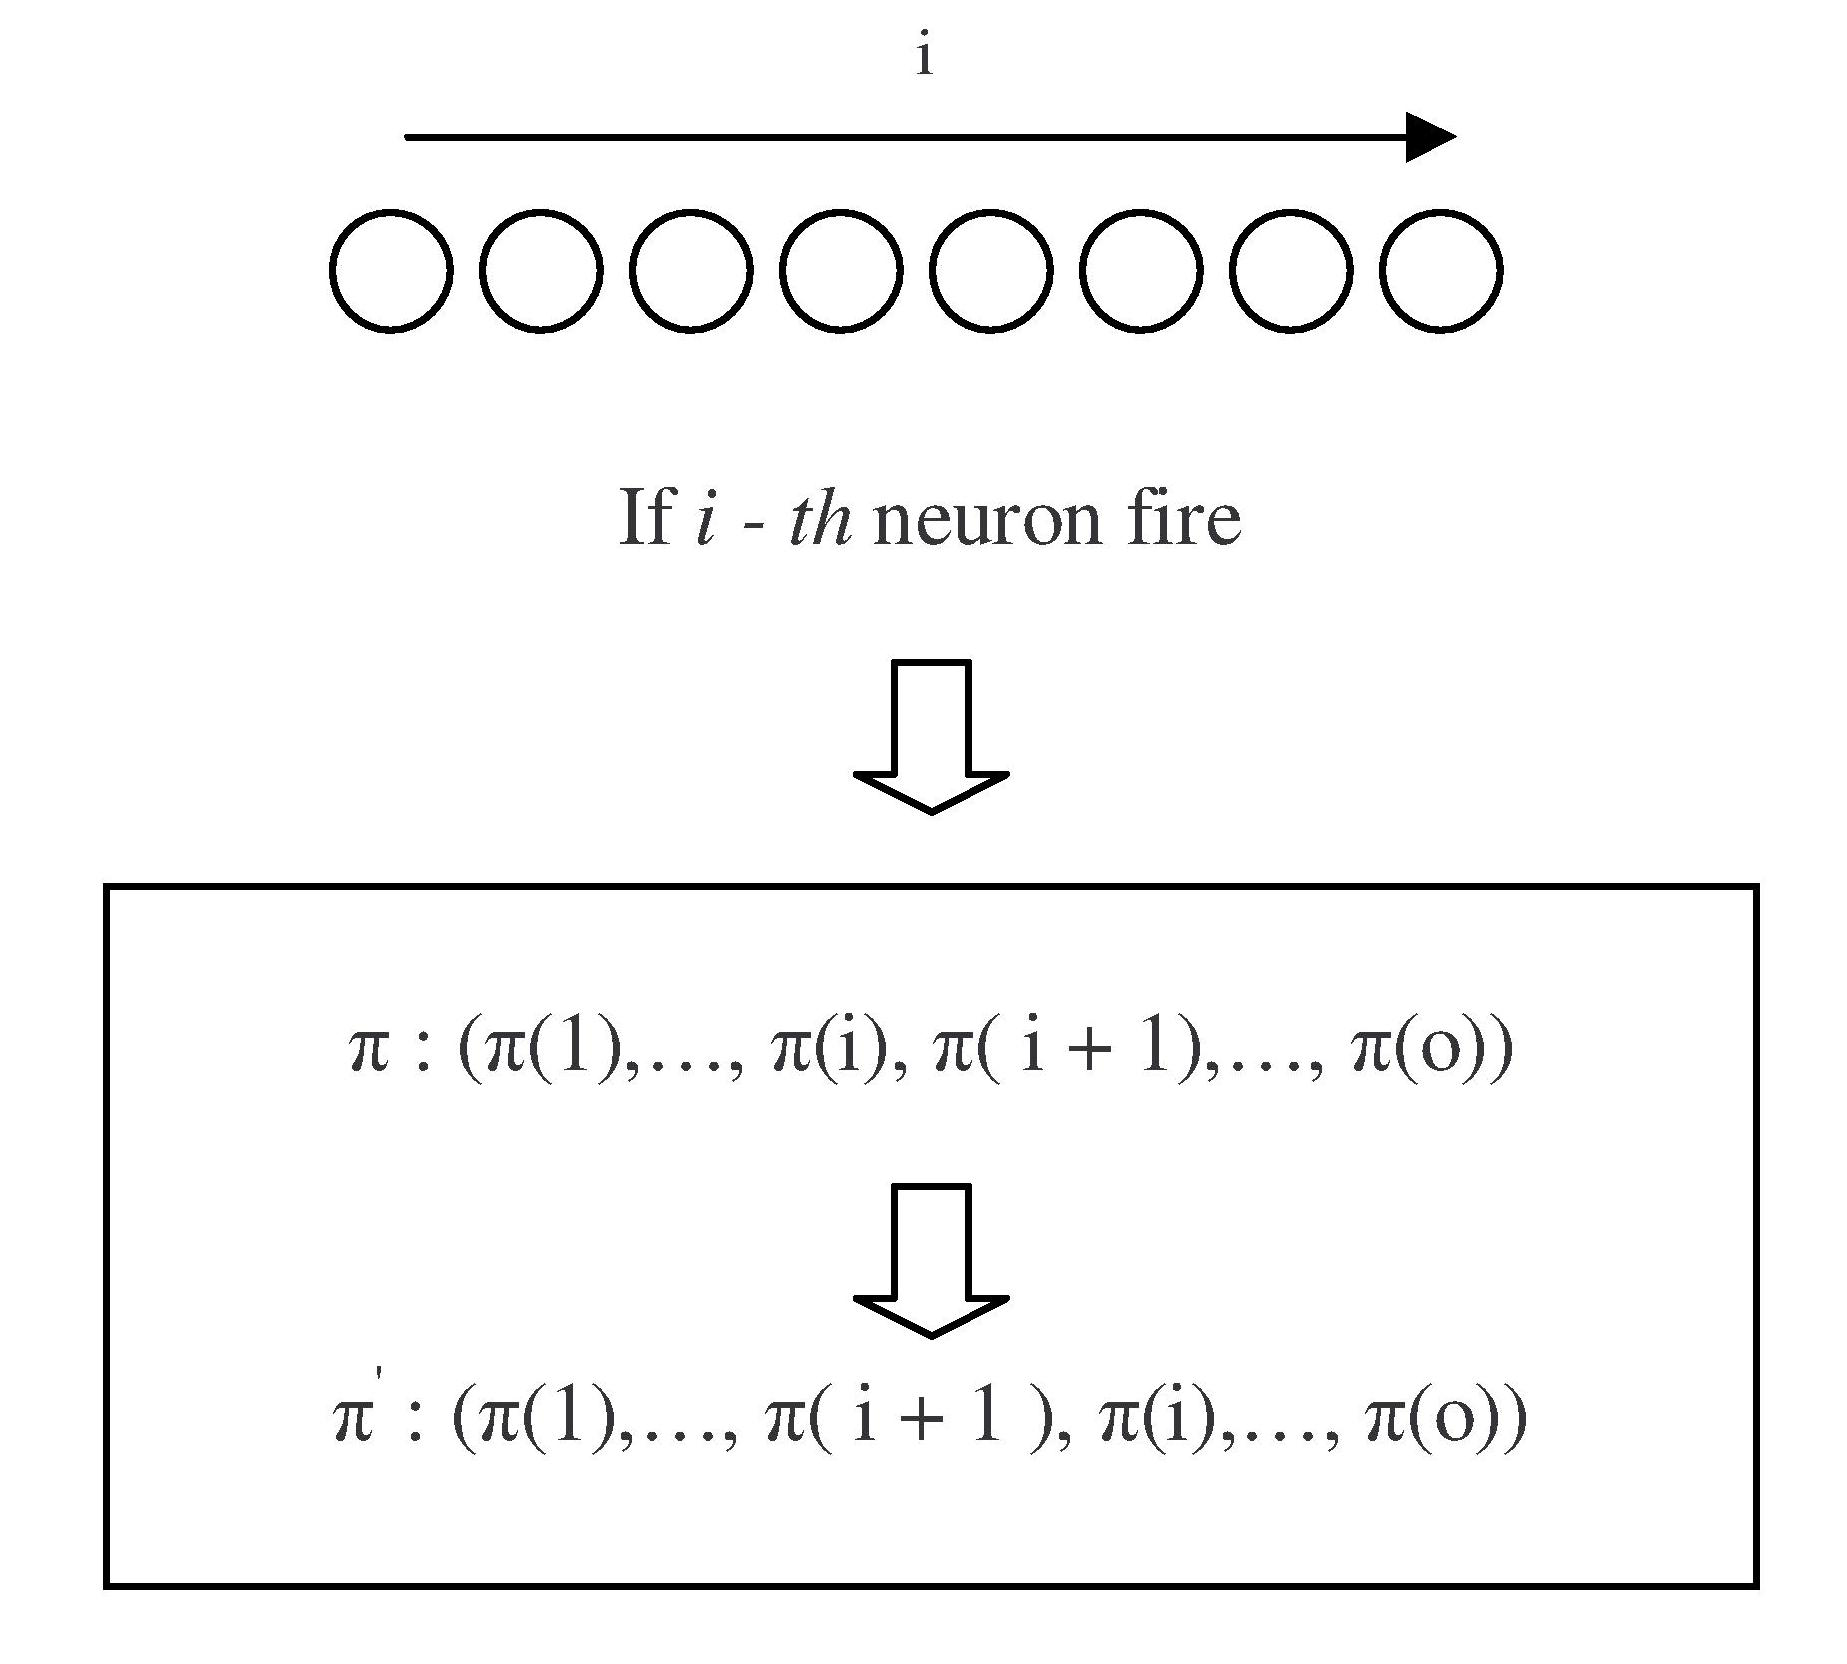
\includegraphics[width=50mm]{neuron_eng.jpg}
\end{figure}

\end{frame}



\subsection{Tabu effect}

\begin{frame}
\frametitle{Tabu effect}

In a proposed neural network architecture a history of each neuron
is stored as its internal state (\textit{tabu effect}). Each neuron is defined by the following
equations:
%
$$
    \eta_{i}(t+1)=\alpha\Delta_{i}(t),
$$
%
$$
    \Delta_{i}(t)=\frac{C_{max}(\pi_{\upsilon}^{(t)})-C_{max}^{*}}{C_{max}^{*}},
$$
%
$$
    \gamma_{i}(t+1)=\sum_{d=0}^{s-1}k^{d}x_{i}(t-d),
    \label{tabu}
$$
where $x_{i}(t)$ is an output of the neuron $i$ in the iteration
$t$.

\end{frame}

\begin{frame}
\frametitle{Tabu effect}

A neuron $i$ is activated if it has the lowest
$\left(\eta_{i}(t+1) + \gamma_{i}(t+1)\right)$ value of all the neurons.
\begin{center}
\begin{figure}[!h]
    \centering
    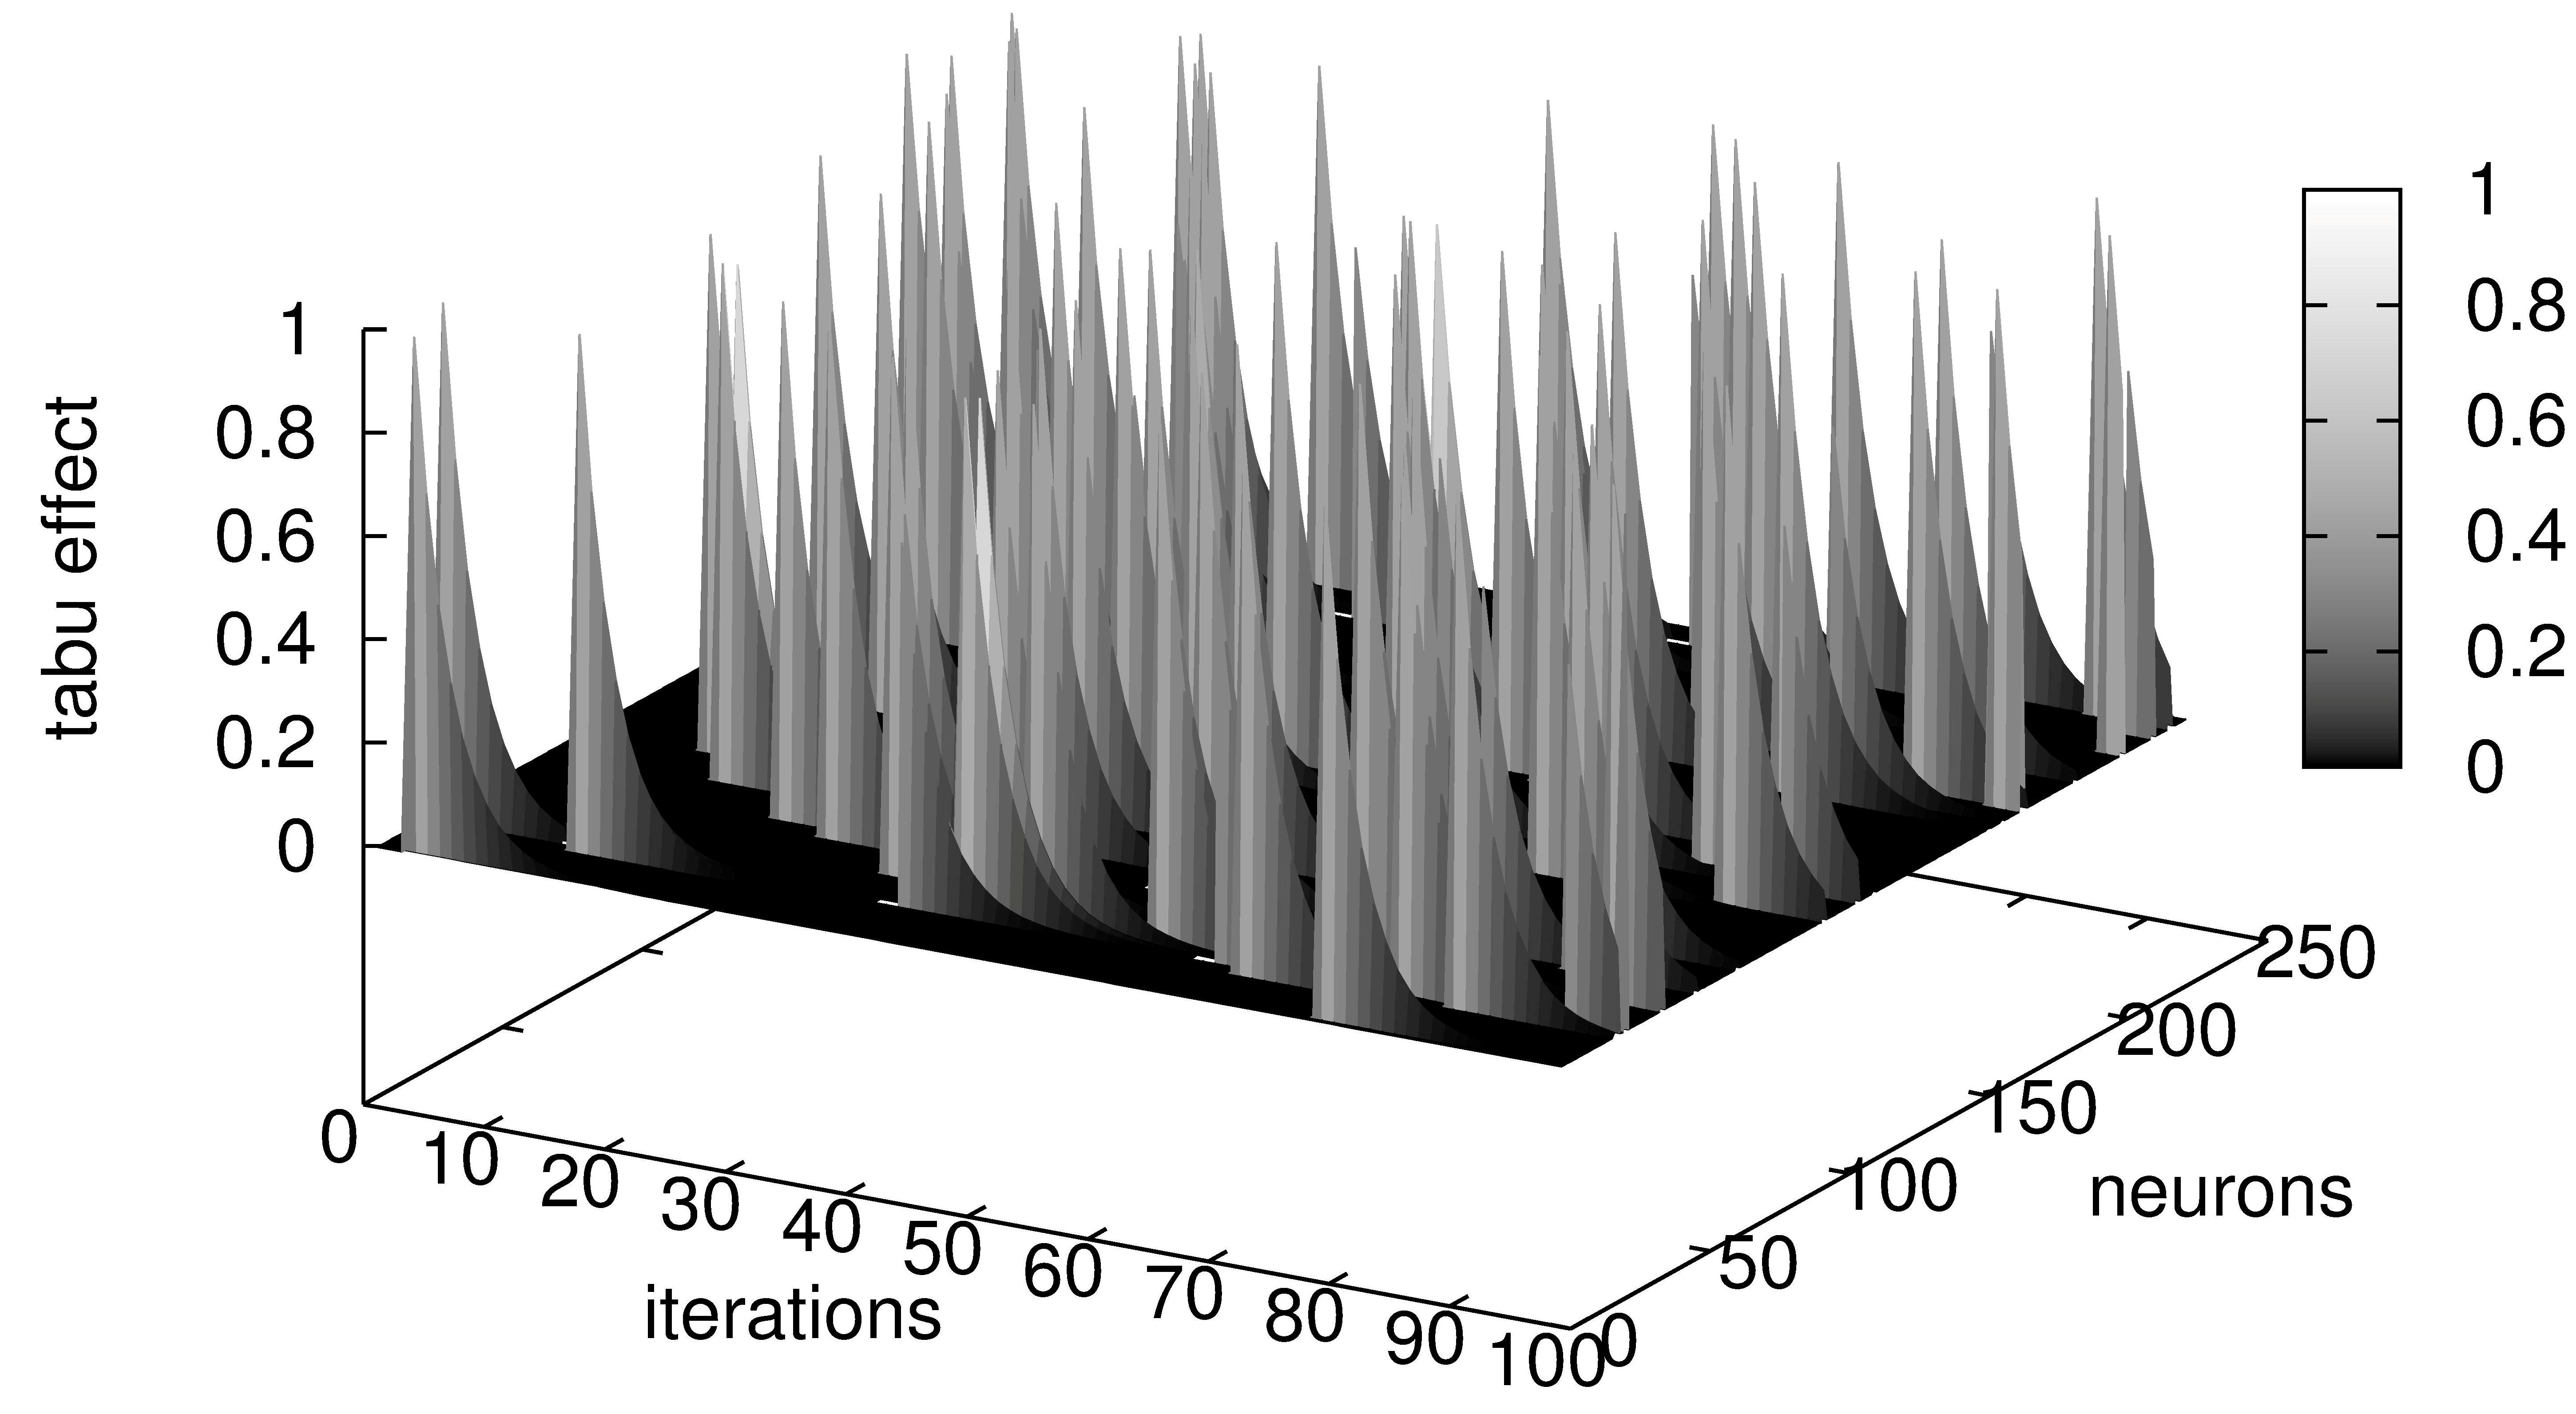
\includegraphics[width=10cm]{tabu_effect.jpg}
\end{figure}
\end{center}

\end{frame}

\section{Parallel neuro-tabu search}

\begin{frame}
\frametitle{Parallel neuro-tabu search}

Here we propose a solution method to the job shop problem
in the distributed computing environments,
such as multi-GPU clusters. Neuro-tabu search algorithm is executed in
concurrent working threads. 

\begin{center}
\begin{figure}[!h]
    \centering
    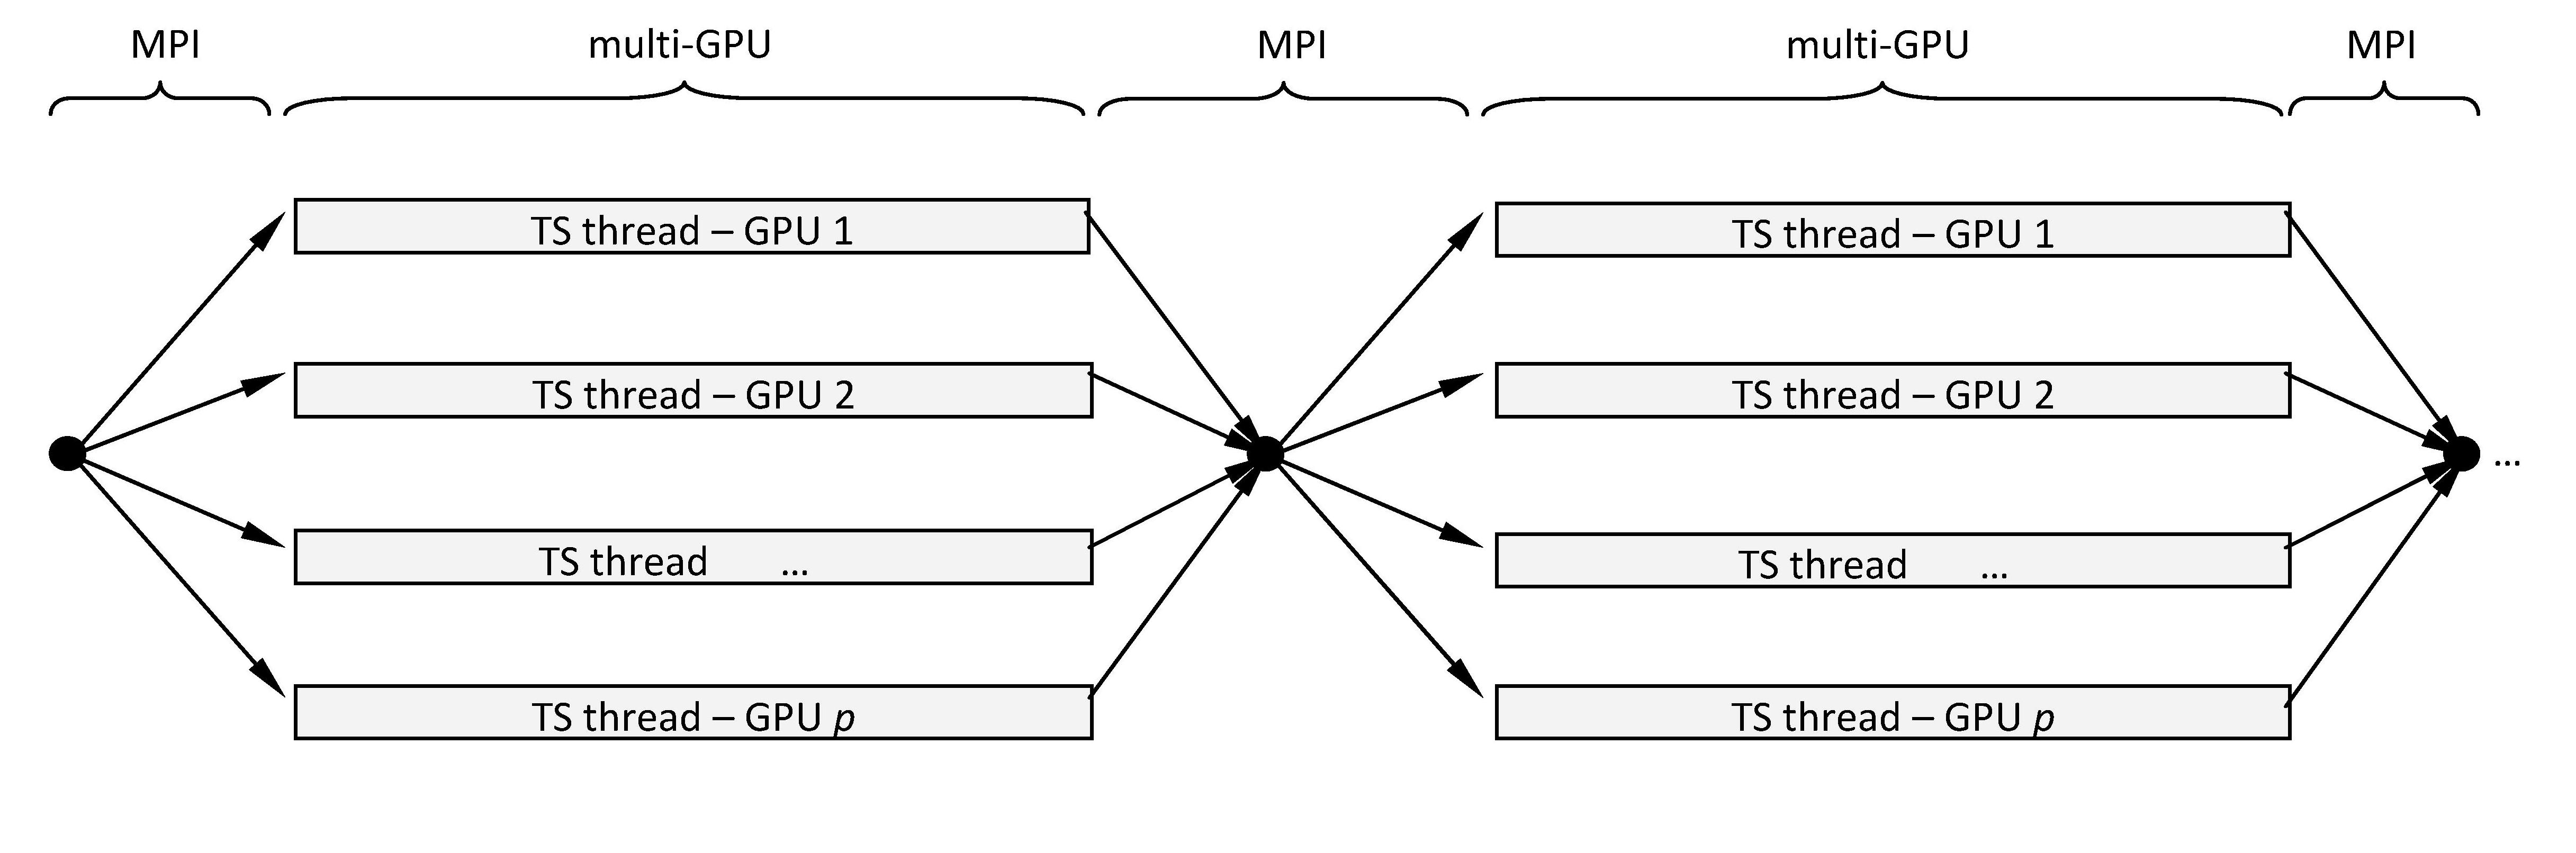
\includegraphics[width=11cm]{multiGPU.jpg}
\end{figure}
\end{center}

\end{frame}

\subsection{Diversification algorithm}

\begin{frame}


\begin{figure}[h!]
\begin{center}
\noindent\framebox[11cm][l]{
\noindent \begin{tabular}{p{105mm}}

\textbf{\tt Algorithm 1. $NIS(\gamma, \delta, C^R)$}\\


%\noindent \begin{tabular}{|l|} \hline


    \textbf{\tt Input:} $\gamma, \delta$ --  two processing orders; $C^R$ -- reference makespan;\\

    \textbf{\tt Output:} $\varphi$ -- processing order; update reference makespan $C^R$;\\

\quad\textbf{\tt $\pi \leftarrow \gamma$; $iter \leftarrow 0$. Find $\delta^{-1}$ and $D(\gamma,\delta)$}\\

\quad\textbf{\tt repeat}\\

\qquad\quad {\tt $iter \leftarrow iter+1$; Find $N(\pi)$;}\\

\qquad\quad {\tt For any $v \in N(\pi)$ calculate and store $C_{max}(\pi_{(v)})$;}\\

\qquad\quad {\tt Find $N^+=\{v=(x,y)\in N(\pi): \delta^{-1}(y)<\delta^{-1}(x)\};$}\\

\qquad\quad {\tt if $N^+ \neq \emptyset$ than $K \leftarrow N^+$ else $K \leftarrow N(\pi)$;}\\

\qquad\quad {\tt Select the move $w \in K$ such, that }\\

\qquad\quad\quad\quad {\tt $C_{max}(\pi_{(w)})=\min_{v \in K} C_{max}(\pi_{(v)})$;}\\

\qquad\quad {\tt Denote $\pi_{(w)}$ by $\alpha$; $\pi \leftarrow \alpha$; $\varphi \leftarrow \pi$;}\\

\qquad\quad {\tt if $C_{max}(\pi) < C^R$ than $C^R \leftarrow C_{max}(\pi)$ and exit;}\\

\quad\textbf{\tt until $iter \geq maxV \cdot D(\gamma,\delta)$; \{$maxV \in (0,1)$ - parameter\}}\\

\end{tabular}

} 
\end{center}
\end{figure}

\end{frame}

\subsection{Intensification algorithm}

\begin{frame}

\begin{figure}[h!]
\begin{center}
\noindent\framebox[11cm][l]{
\noindent \begin{tabular}{p{105mm}}

\textbf{\tt Algorithm 2. $iNTS$}\\


%\noindent \begin{tabular}{|l|} \hline


\textbf{\tt Input:} $\pi^0$ --  processing orders provided by INSA; \\

\textbf{\tt Output:} $\pi^*$ -- the best found processing order\\

\quad\quad\quad\quad\quad\quad     and its makespan $C^*$;\\

\quad\textbf{\tt $(\pi^1,C^1) \leftarrow NTS(\pi^0)$; $C^* \leftarrow C^1$;}\\

\quad\textbf{\tt for $i \leftarrow 2,\ldots,maxE$ do}\\

\qquad\quad {\tt $\varphi \leftarrow NIS(\pi^{i-1},\pi^0,C^*)$; $(\pi^i,C^i) \leftarrow NTS(\varphi)$;}\\

\qquad\quad {\tt $C^* = \min\{C^*,C^i\}$;}\\

\quad\textbf{\tt repeat}\\

\qquad\quad {\tt Find $1 \leq l \leq maxE$ so that }\\

\qquad\quad\quad {\tt $D(\pi^k,\pi^l) = \max \{D(\pi^k,\pi^i):1 \leq i \leq maxE\}$; }\\

\qquad\quad\quad {\tt $\varphi \leftarrow NIS(\pi^k,\pi^l,C^*)$; $(\pi^l,C^l) \leftarrow {\bf NeuroTS}(\varphi)$;}\\

\qquad\quad {\tt if $C^l < C^k$ than set $(\pi^*,C^*) \leftarrow (\pi^l,C^l)$ and $k \leftarrow l$;}\\

\quad\textbf{\tt until $\max\{D(\pi^k,\pi^i):1 \leq i \leq maxE\} < maxD$.}\\

\end{tabular}

} 
\end{center}
\end{figure}

\end{frame}



\section{Computational experiments}

\begin{frame}
\frametitle{Computational experiments}

Proposed algorithms were ran on the server based on 6-cores Intel Core i7 CPU X980 (3.33GHz) processor equipped with nVidia Tesla S2050 GPU (1792 cores).
% working under 64-bit GNU/Linux Ubuntu 10.10
%operating system. Notion used:
\begin{itemize}
\item $sNTS$ -- sequential neuro-tabu Search algorithm,
\item $pNTS$ -- parallel (for $p=16$) neuro-tabu Search algorithm, 
\item $iNTS$ -- advanced $NTS$ algorithm based on the diversification and intensification methodology.
\end{itemize}

\begin{center}
\begin{figure}[!h]
    \centering
    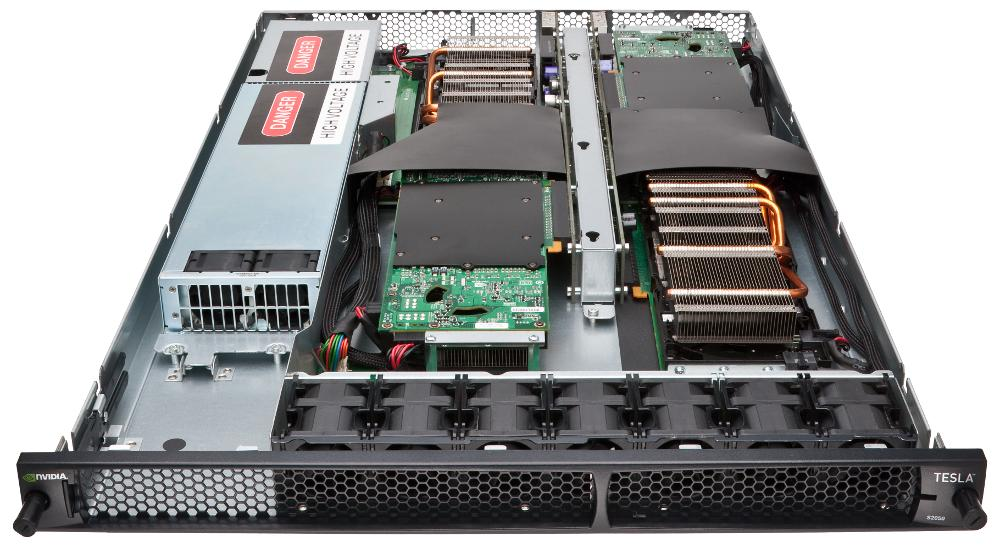
\includegraphics[width=57mm]{Tesla_S2050.jpg}
\end{figure}
\end{center}

\end{frame}

\begin{frame}
\frametitle{Results of experiments}

\begin{table}[h]
\centering
\begin{tabular*}{0.9\textwidth}{@{\extracolsep{\stretch{1}}}ccccc}\hline
problem & $n \times m $  & $sNTS$  & $pNTS$($p=16$) & $iNTS$ \\
\hline
TA01-10 & $15\times 15 $    & 0.4948 & 0.3141 & 0.0652  \\
TA11-20 & $20\times 15 $    & 1.1691 & 0.9129 & 0.4412  \\
TA21-30 & $20\times 20 $    & 1.2486 & 0.7033 & 0.4803  \\
TA31-40 & $30\times 15 $    & 1.0592 & 0.7965 & 0.3764  \\
TA41-50 & $30\times 20 $    & 1.8565 & 1.5634 & 0.8328  \\
TA51-60 & $50\times 15 $    & 0.0915 & 0.0915 & 0.0520  \\
TA61-70 & $50\times 20 $    & 0.1479 & 0.0210 & 0.0140  \\
TA71-80 & $100\times 20 $   & 0.0090 & 0.0090 & 0.0090  \\\hline
\multicolumn{2}{c}{\bf average} & {\bf 0.7596} & {\bf 0.5515} & {\bf 0.2839}  \\\hline
\end{tabular*}
\caption{Percentage relative deviations (PRD) to the best known
solutions.\label{tab}}
\end{table}

\end{frame}


\section{Conclusions}


\begin{frame}
\frametitle{Conclusions}

\begin{itemize}
\item We propose an approach designed to solve difficult problems
of combinatorial optimization in distributed parallel architectures without
shared memory, such as clusters of nodes equipped with GPU units (i.e. multi-GPU clusters).

\item The methodology can be especially effective for large instances of hard to solve optimization problems,
such as flexible scheduling problems as well as discrete routing and assignment problems.
\end{itemize}

\end{frame}

\end{document}












\section{Computational experiments}

\begin{frame}
\frametitle{Computational experiments}

The main part of our parallel implementation of goal function
calculation for the job shop problem constitute calculating of the
longest path between all vertexes in graph. This part was
parallelized with CUDA and OpenCL and ran on NVidia and ATI GPUs.
We run our algorithm on three different GPUs:
\begin{itemize}
\item NVidia GTX480 with 480 parallel processor cores and 1.4 GHz
clock rate, \item ATI Radeon HD5870 with 20 compute units and 850
MHz clock rate, \item ATI Radeon HD5970 with 20 compute units and
725 MHz clock rate.
\end{itemize}

This GPUs are installed in servers with Intel Core i7 CPU with
3.20 GHz clock rate working under 64-bit GNU/Linux Ubuntu 10.10
operating system.

\end{frame}



\subsection{Conclusions}

\begin{frame}
\frametitle{Conclusions}
\begin{itemize}
\item In this work we have shown the method of parallelization of
the job shop problem solving algorithm for GPGPU, consisting in
parallelization of the cost function calculations.

\item The proposed algorithm can be used for computation
acceleration in metaheurisics solving the job shop problem.

\item The calculation time of goal function in algorithms which
solve the job shop problem take even 90\% of the whole algorithm
computation time.

\item The use of parallel algorithm for goal function calculation
might result in significant decreasing of algorithm execution time
for solving the job shop problem.

\end{itemize}


\end{frame}
